\documentclass[a4paper,11pt,parskip=never,DIV=8,chapterprefix=true,titlepage=true,twoside,twocolumn,open=any]{scrbook}
%\usepackage{mathptmx}% http://ctan.org/pkg/times
\usepackage{tgpagella}
%\usepackage[osf,sc]{mathpazo}% http://ctan.org/pkg/times
%\usepackage[sc]{mathpazo}% http://ctan.org/pkg/times
\linespread{1.05}
\setcounter{secnumdepth}{0}
\renewcommand*\sectfont{\normalcolor\bfseries}% removed \sffamily
%\setparsizes{1em}{0.25\baselineskip plus .25\baselineskip}{1em plus 1fil} 
\usepackage[T1]{fontenc}
\usepackage{textcomp} % provide euro and other symbols
\usepackage[labelformat=empty,font=small]{caption}
\usepackage{float}
\usepackage{caption}
\usepackage{amsmath}
\usepackage{amssymb}
\usepackage{microtype}
\usepackage{lettrine}
\usepackage[export]{adjustbox}
\usepackage{graphicx}
\usepackage{xcolor}
\usepackage{booktabs}
\usepackage{enotez}
\usepackage[english]{babel}
\usepackage{blindtext}
\usepackage{lipsum}
\usepackage{verse}
\usepackage{bibleref}
\setlength{\columnsep}{.7cm}
\addtokomafont{title}{\Huge}
\addtokomafont{section}{\normalsize}
\addtokomafont{subsection}{\normalsize}
\usepackage{balance}
\usepackage{makeidx}
%\usepackage{showframe}
%\usepackage[showframe]{geometry}
\usepackage{geometry}
\usepackage{enumitem}
\setitemize{noitemsep,topsep=0pt,parsep=0pt,partopsep=0pt}
\renewcommand\labelitemi{$\vcenter{\hbox{\tiny$\bullet$}}$}
\AfterCalculatingTypearea{\geometry{margin=2cm,top=3cm,bottom=3.5cm,bindingoffset=6mm}}
%\AfterCalculatingTypearea{\geometry{margin=2.5cm,top=5cm,bottom=5cm,bindingoffset=12mm,nofoot}}
\recalctypearea
%\captionsetup{belowskip=.25em,aboveskip=1em}
\renewcommand\topfraction{0.85}
\renewcommand\bottomfraction{0.85}
\renewcommand\textfraction{0.1}
\renewcommand\floatpagefraction{0.85}

%\pretolerance=8000
%\tolerance=1000
%\emergencystretch=-1pt
%\righthyphenmin=4
%\lefthyphenmin=4

%\usepackage[showframe]{geometry}
%\usepackage{geometry}
%\usepackage[%
%  a4, % <===============================================================
%  axes,cross,pdftex,center
%]{crop}

\DeclareInstance{enotez-list}{plain}{paragraph}{notes-sep=0pt}
\LettrineRealHeighttrue


\setenotez{
  reset=true,
  list-name=Endnotes,
  list-heading = \section*{#1},
  backref=true,
  list-style=plain
}

\DeclareInstance{enotez-list}{custom}{paragraph}
{
%format = \small ,
%format = \footnotesize ,
format = \scriptsize\raggedright, 
%format = \tiny ,
notes-sep=0pt,
number = \textsuperscript{#1}
}
\let\footnote=\endnote
%\usepackage{biblatex}
%\usepackage{chapterbib}
\usepackage{import}
\usepackage{wrapfig}
\usepackage{upquote}
%\usepackage{bookmark}
%\usepackage{hyperref}
\usepackage{nicefrac}
\usepackage[noabbrev]{cleveref}
\usepackage[headsepline=true, autooneside=false]{scrlayer-scrpage}

\makeindex

\pagestyle{scrheadings}

\lohead{}
\cohead{}
\rohead{\leftmark}

\cofoot[]{}
\rofoot[\pagemark]{\pagemark}

\automark[section]{chapter}

\begin{document}

\begin{titlepage}
\par\vspace*{.15\textheight}
\begin{center}
\vskip 1em
{\fontsize{50}{60}\selectfont
Christ Church

\vspace{5mm}
Murgon
}
\vskip 2em
{\fontsize{20}{30}\selectfont
Celebrating 100 Years\\

\vspace{2mm}
of Anglican Parish History
}
\vfill
{%
\usekomafont{author}{ Compiled By Marcia McIntosh \par}%
}%
\end{center}

\clearpage
\thispagestyle{empty}
\noindent\begin{minipage}[t]{\textwidth}
{\small Printed By:\\T J Printing Group\\42 King St, Deception Bay QLD 4508}
\end{minipage}\par
\par\vspace*{.35\textheight}
\noindent\begin{minipage}[b]{\textwidth}
\begin{center}
{\small In the spirit of reconciliation we acknowledge the Traditional Custodians
of country throughout Australia and their connections to land, sea and community.
We pay our respect to their elders past and present and extend that respect to all
Aboriginal and Torres Strait Islander peoples today.}
\end{center}
\end{minipage}\par
\vfill
\noindent\begin{minipage}[b]{\textwidth}
\noindent\begin{minipage}[b]{.45\textwidth}%

\includegraphics[width=\linewidth,left]{../images/nlaLogo.jpg}
\end{minipage}%

\bigskip\noindent
ISBN 978-0-646-83551-8 	

\bigskip\noindent
\copyright{ }Marcia McIntosh, 2021

\bigskip\noindent
{\small This book was set with the help of {\KOMAScript} and {\LaTeX}}
\end{minipage}\par

\clearpage
\thispagestyle{empty}
\par\vspace*{.1\textheight}
\noindent\begin{minipage}[t]{\textwidth}
\begin{center}
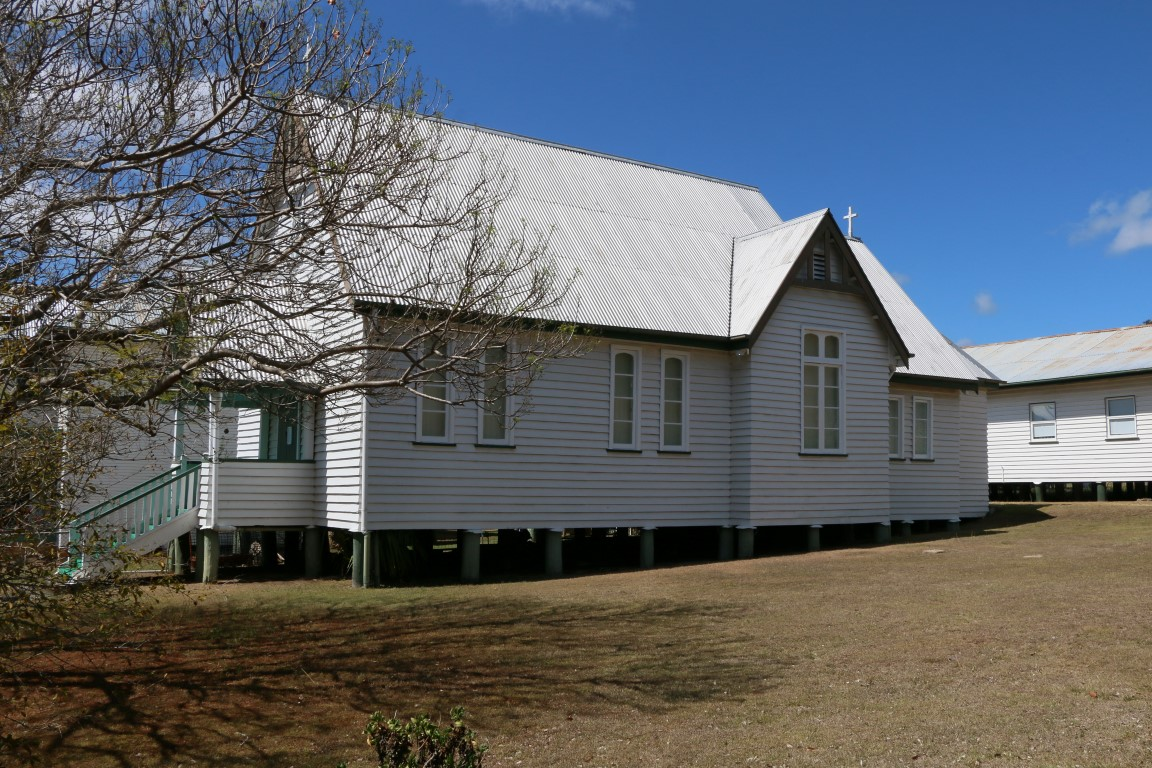
\includegraphics[width=.85\linewidth,center]{../images/christChurchMurgon_2019_11_29.jpg}
\end{center}
\end{minipage}\par
\vspace{5mm}
\noindent\begin{minipage}[b]{\textwidth}
\begin{center}
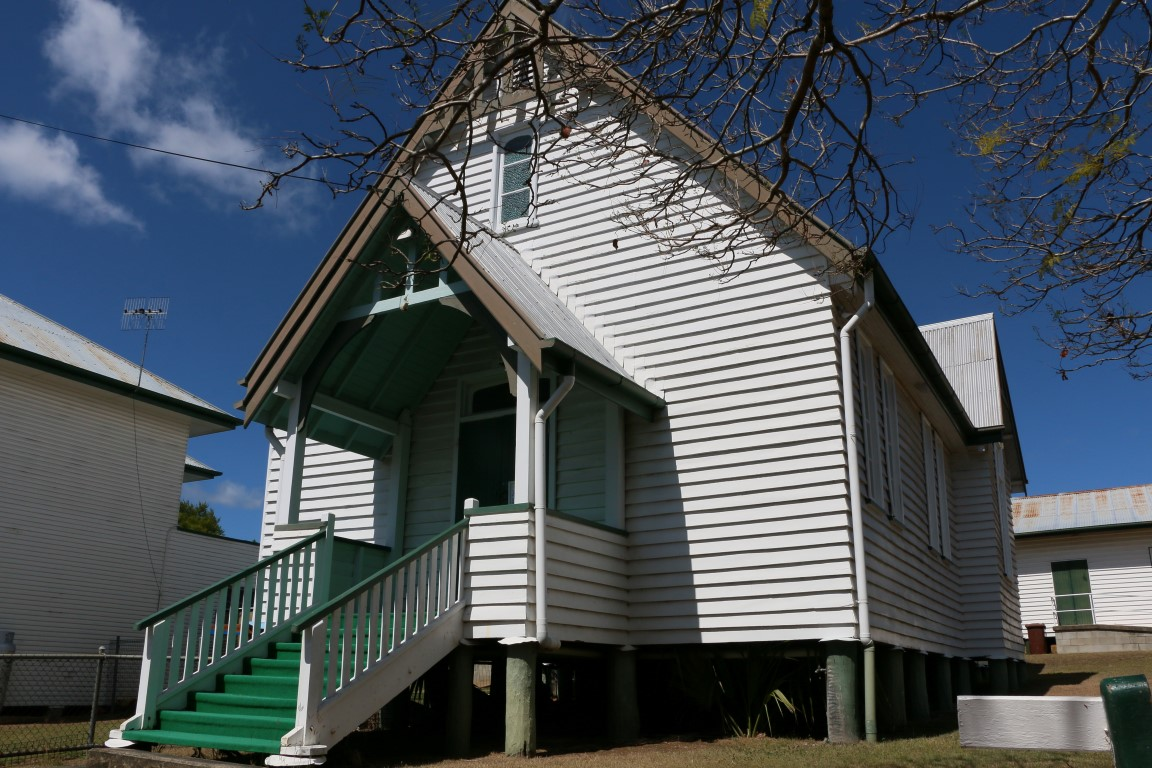
\includegraphics[width=.85\linewidth,center]{../images/christChurchMurgon_front_1_2019_11_29.jpg}
{\small {\itshape Christ Church Murgon, 2019} {\small(Ruth Kerr)}}
\end{center}
\end{minipage}
\newpage
\thispagestyle{empty}
\par\vspace*{.1\textheight}
\noindent\begin{minipage}[t]{\textwidth}
\begin{center}
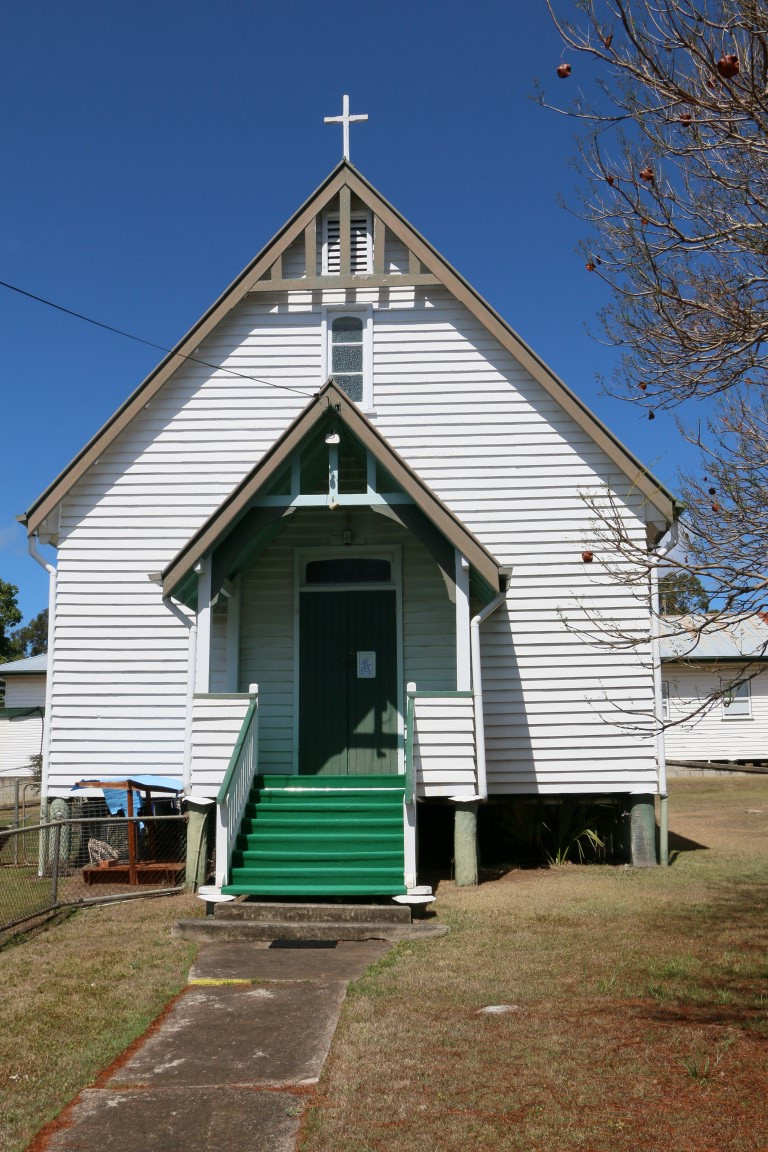
\includegraphics[width=.8\linewidth,center]{../images/christChurchMurgon_front_2019_11_29.jpg}
{\small {\itshape Christ Church Murgon, 2019} {\small(Ruth Kerr)}}
\end{center}
\end{minipage}\par

%  \clearpage
%  \thispagestyle{empty}
%  \par\vspace*{.45\textheight}
%  \noindent\begin{minipage}[b]{\textwidth}
%  \begin{center}
%    {\small In the spirit of reconciliation we acknowledge the Traditional Custodians
%            of country throughout Australia and their connections to land, sea and community.
%            We pay our respect to their elders past and present and extend that respect to all
%            Aboriginal and Torres Strait Islander peoples today.}
%  \end{center}
%  \end{minipage}\par
\end{titlepage}
%\newpage
\onecolumn
\frontmatter

%\setchapterpreamble[o]{
%\dictum[Psalm 56:3]{But when I am afraid,\linebreak I will put my trust in you.}}

%\cleardoublepage
\chapter{Foreword}


\lettrine[lines=3]{T}{HE} Centenary of the dedication of Christ Church Murgon is reason to pause and 
give thanks to God for the ministry of the church in this place. Many stories 
are recorded in this history compiled by Marcia McIntosh.
\smallskip

\noindent
This sacred space, in which countless baptisms, weddings and funerals have taken 
place over the years, as well as services of Morning and Evening Prayer and Holy 
Communion, is held high in the affections of many people across the generations.  
\smallskip

\noindent
Who can number the blessings that have flowed in people's lives because of the 
ministry of Christ Church Murgon? Times of joy and times of sadness, all have been 
held before God in the name of Christ, in the light of the gospel. The sacraments 
of the church have incorporated and strengthened generations. 
\smallskip

\noindent
We can but praise God for ministry in this place, for the people who have worshipped 
here and for the clergy who have been called to serve here and lives which have 
been renewed and restored here.

\smallskip

\noindent The words of Psalm 84 are apt:
\smallskip

\begin{center}
\begin{minipage}[b]{.6\linewidth}%
{\itshape
\noindent 1 How lovely is your dwelling-place:\\
\hphantom{MM}O Lord God of hosts!

\noindent 2 My soul has a desire and longing\\
\hphantom{MM}to enter the courts of the Lord:\\
\hphantom{MM}my heart and my flesh rejoice in the living God.

\noindent 3 The sparrow has found her a home,\\
\hphantom{MM}and the swallow a nest where she may lay her young:\\
\hphantom{MM}even your altar, O Lord of hosts,my King and my God.

\noindent 4 Blessed are those who dwell in your house\\
\hphantom{MM}they will always be praising you.
}
\end{minipage}%
\end{center}


\bigskip

\noindent
\begin{minipage}[b]{1.1\linewidth}%
\begin{minipage}[b]{0.70\linewidth}%

I commend to you this account of the generations who have encountered God through 
Christ Church Murgon.

\smallskip
Thanks be to God for the enduring witness of so many faithful people who have worshipped here. 
May transforming encounters with God in Christ continue in this place for many generations to come.

\vspace{1cm}%
\noindent The Most Reverend Dr Phillip Aspinall

\vspace{5mm}%
\noindent Archbishop of Brisbane
\end{minipage}%
\hspace{2em}
\begin{minipage}[b]{.19\linewidth}%
\begin{center}%
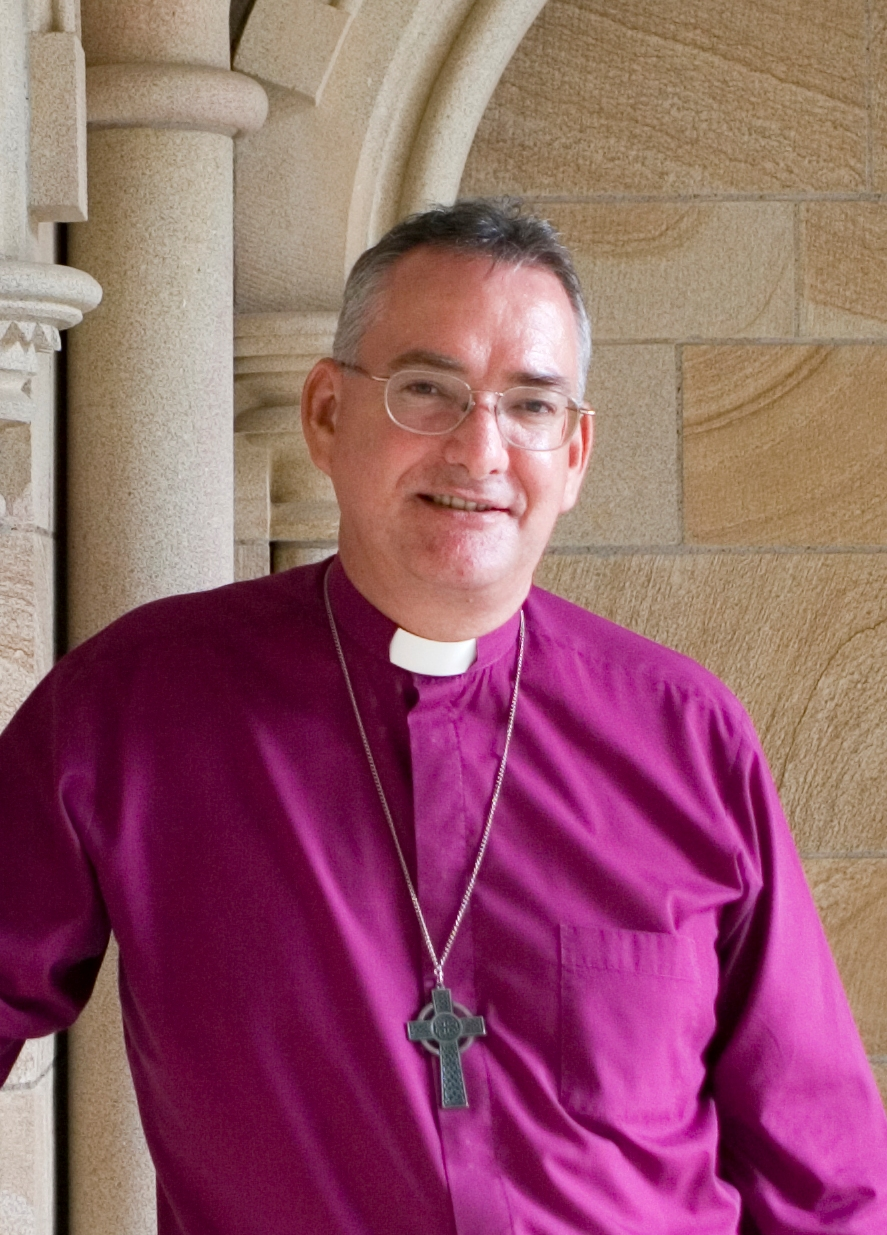
\includegraphics[width=\linewidth,right]{../images/abpPhoto.jpg}
\end{center}%
\end{minipage}%
\end{minipage}%

{
\setcounter{tocdepth}{2}
\tableofcontents
}

\twocolumn
\mainmatter
\setcounter{page}{1}

\setchapterpreamble[o]{
\dictum[Matthew 17:7]{And Jesus came and touched them, and said, Arise, and be not afraid.}}

\chapter{Introduction}
\lettrine[lines=3]{T}{HE} Murgon parish has grown from a dream in the minds of the 
European settlers who arrived after the opening of the railway in 1903 - timber getters, 
selectors, business people - who all developed the town of Murgon and surrounding 
districts. External factors - wars, depressions, weather conditions, advent of personal 
ownership of the motor car, and changing societal responses to organised religious 
observance - have influenced the role of the Murgon's Christ Church Anglican Church 
in the Barambah Parish. 

Murgon is a new town in comparison with its neighbours, Gayndah and Nanango. Murgon 
town established itself around the railway station. The town and surrounding farms 
were excised from \emph{Barambah}, \emph{Boonara} and \emph{Manumbar} pastoral stations. 
Cherbourg Aboriginal Community was reserved out of \emph{Barambah} and is part of 
the Barambah Parish. The uptake of land selections and town allotments was steady.

\begin{figure}
\begin{center}
\includegraphics[width=1.\linewidth,center]{../images/theAustralianHymnBook.jpg}
\end{center}
\end{figure}

The South Burnett has been a highly productive agricultural region since the arrival 
of European settlers. Group Settlements were organised of young men from northern 
New South Wales, the Fassifern and Lockyer districts and Brisbane before World War I 
seeking opportunities in the new settlements. Extraction of the pine timber on the 
selections provided the financial foundation for establishing productive dairy farms 
and crops. 

These people formed Christian communities and built churches as a priority, formed 
out of the cultural traditions of their ancestors. From as early as 1864 Rev George 
Julius Tatham of Tiaro south of Maryborough, followed by members of the Bush Brotherhood 
operating out of Gayndah, visited the Anglicans in the Murgon region. A more formalized 
arrangement with Curate, Rev J H Steer from Nanango, was introduced in 1903 over the area 
which later became the Parish of Murgon and Kilkivan, leading to the construction of 
Christ Church.  The construction of Christ Church in Murgon was rapid, beginning in 
1919 with funds raised, tenders being let, stump-capping in September 1919 and dedication 
of the unlined building in April 1920 on land purchased and then donated by George and 
Charlotte Arnell for the church.


In 1919 when Christ Church Anglican Parish was formed the priest served the people in 
Murgon, Wondai, Mondure, Sexton, Abbeywood, Silverleaf, West Goomeri, Kilkivan, Boonara, 
Goomeri, Cinnabar, Fat Hen Creek and Barambah Mission, travelling by horseback and later 
a 'Tin Lizzie' Ford car. 

Christ Church Murgon was well sustained for decades by farmers, town business people, 
public servants, trades people, workers at the butter and cheese factories, the railway 
and council workers. 
\balance

The Anglican parishioners and the 18 priests who have served in Murgon have valiantly 
espoused their mission through constant service to the community, fund raising, regular 
patterns of church services, Sunday Schools, Youth Groups, Ladies' Guilds, Mothers Union 
and Men's Groups. I saw all this activity in Murgon in 1969 when I was a parishioner. The 
local agricultural industry was then very prosperous and each Sunday around 40 people gathered 
in Christ Church with Rev Alf Gerlach for the Eucharist service. 

Agriculture continued to prosper in the following 50 years, becoming highly mechanised, 
and young people left the district to embark on higher education. The substantial change 
in the demography and economy of Murgon has been very evident in recent years. Christ Church 
Anglican Parish, along with all the other main line denominations in the town, illustrates the 
evolution of the Church parish model in which church participation has all but disappeared. 
The current challenge is in grasping the opportunity that the stimulation by the pandemic 
to regional repopulation may bring.

\vspace{1cm}
\noindent Dr Ruth S Kerr
\vspace{5mm}

\noindent Member of Diocesan Council

\noindent Anglican Church Southern Queensland

\noindent 22 February 2021

\import{./}{formatted-mainmatter-idx.tex}

\vspace{1.5cm}
\noindent Marcia McIntosh
\vspace{5mm}

\noindent March 2021

\printindex
\end{document}
